\begin{figure}[b!]
\centering
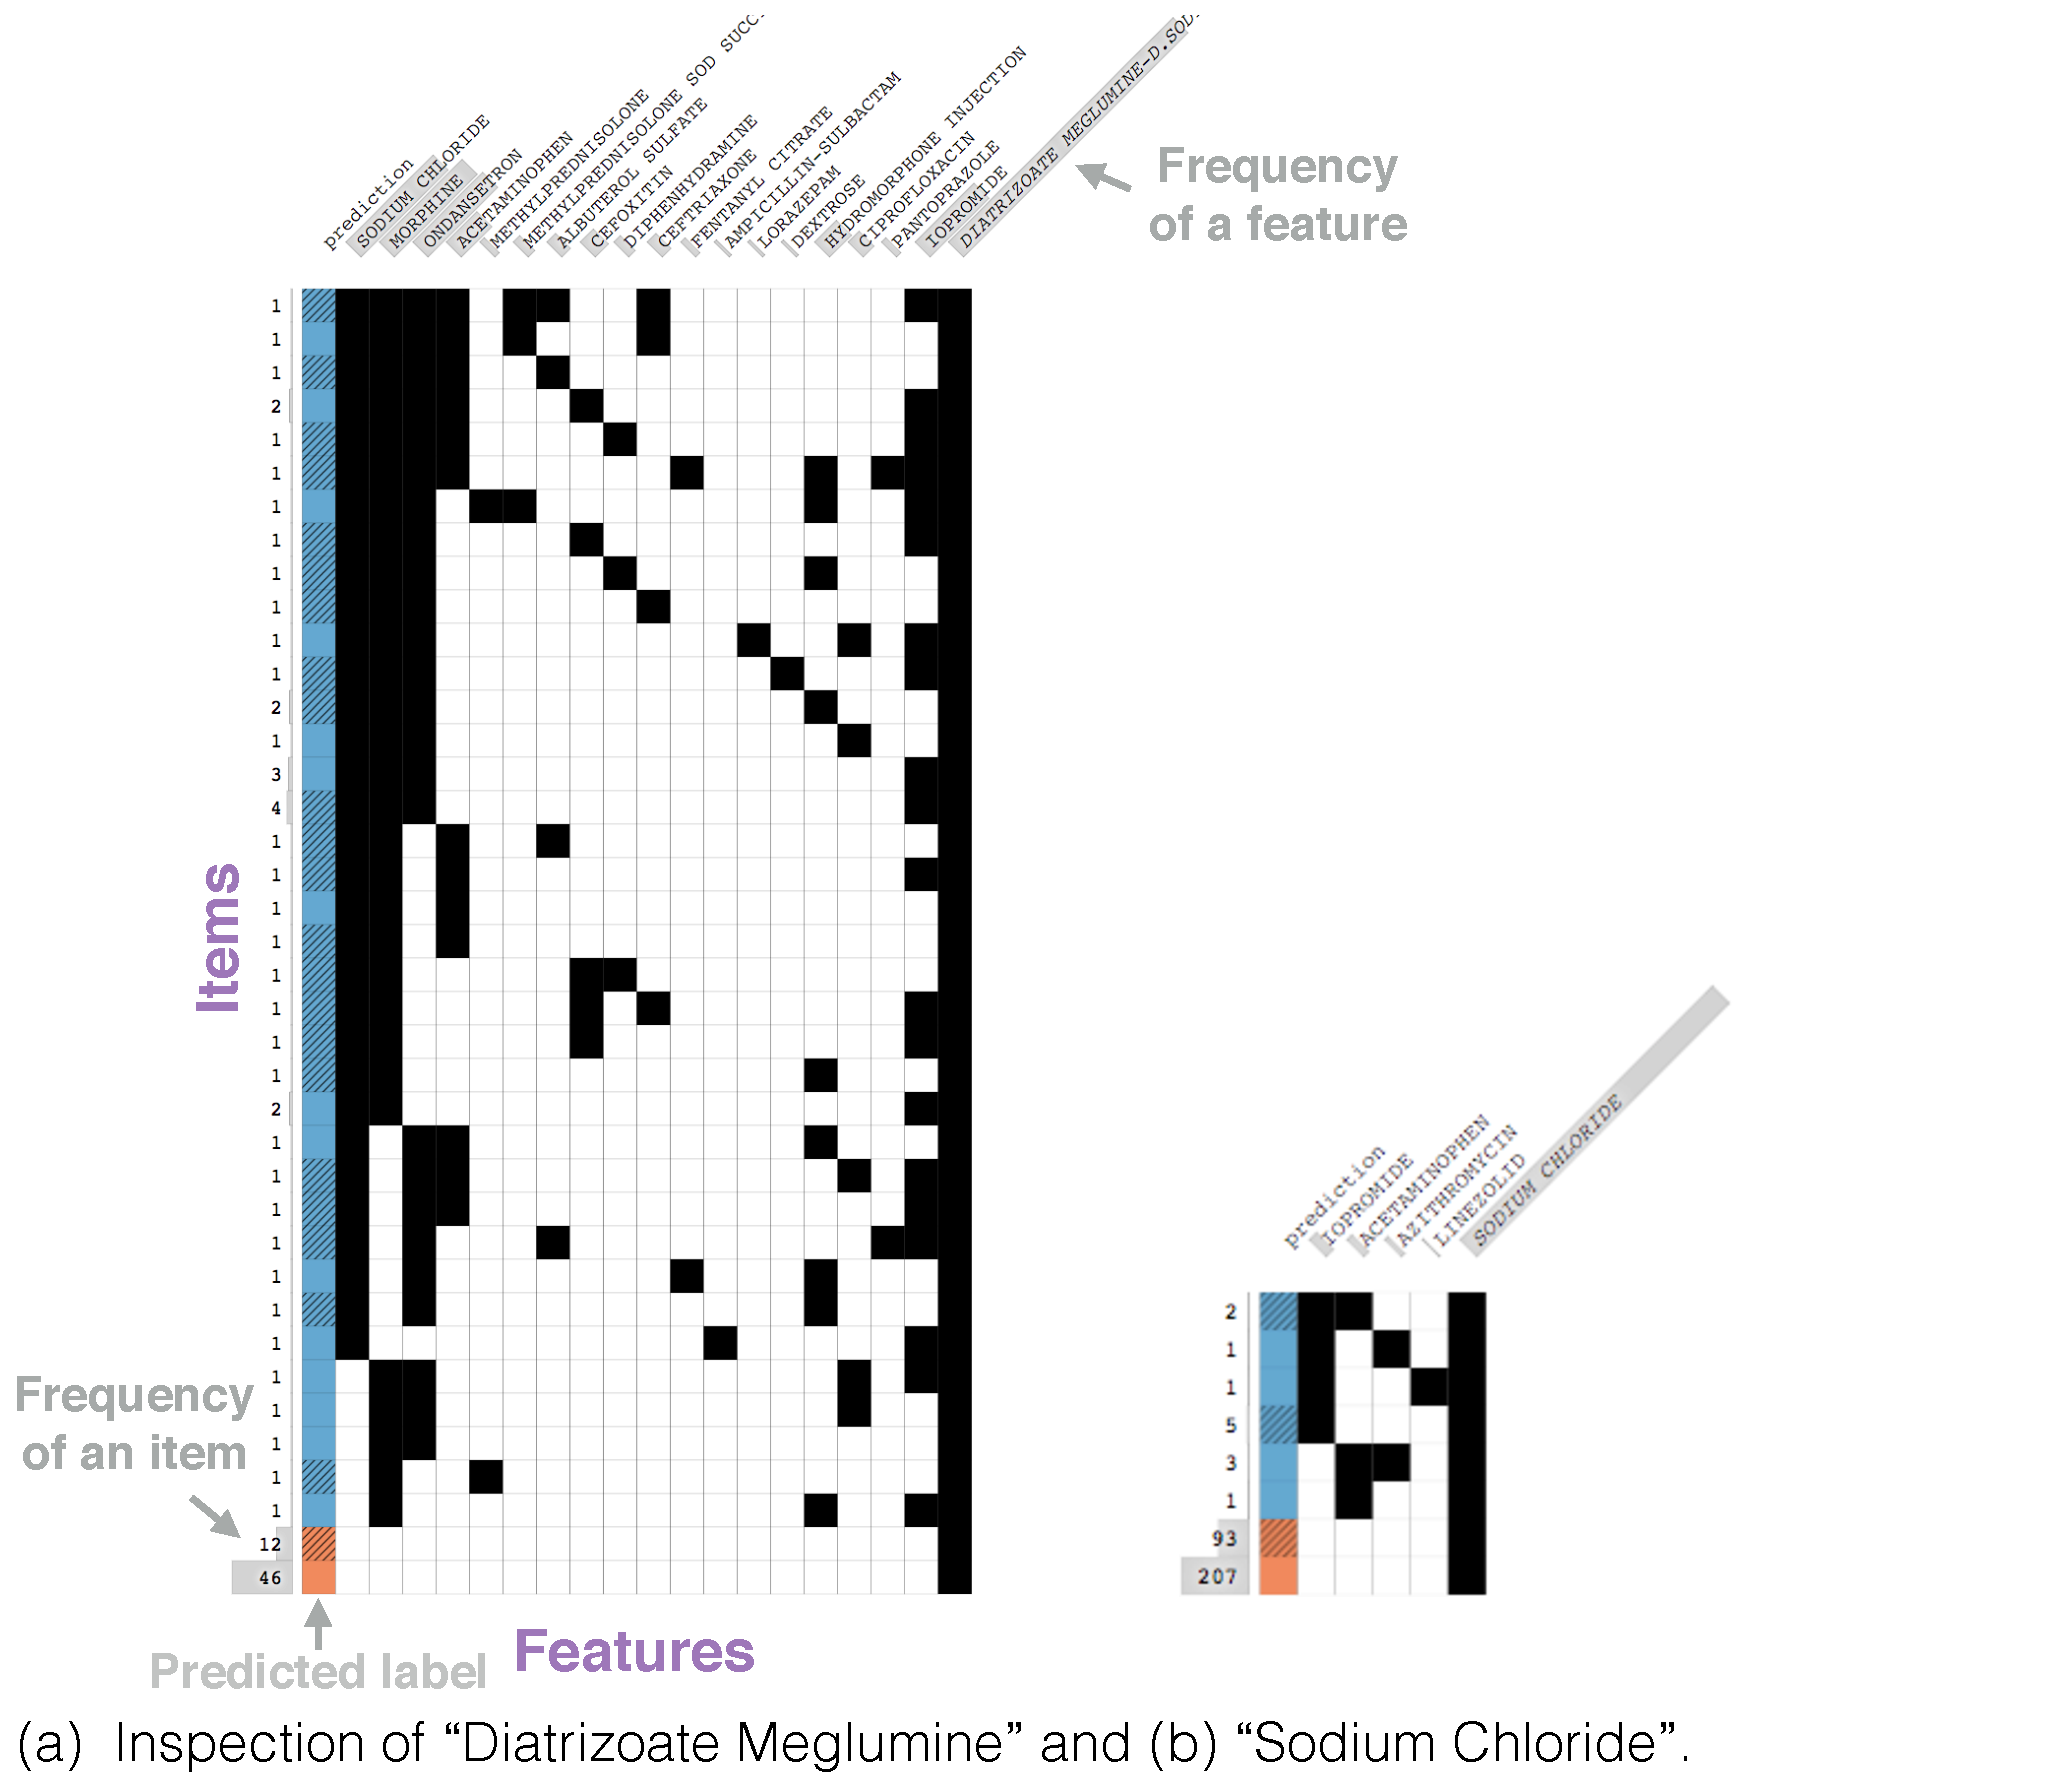
\includegraphics[width=0.9\linewidth]{explainer/inspect1}
% \begin{subfigure}[b]{0.7\linewidth}
%     \centering
%     \includegraphics[width=\linewidth]{fig/inspect}
%     \caption{~Inspection of ``Diatrizoate Meglumine"}
%     \label{figs:inspect}
% \end{subfigure}
% \hspace{-3em}
% \begin{subfigure}[b]{0.35\linewidth}
%     \centering
%     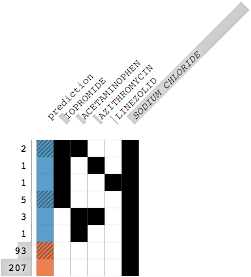
\includegraphics[width=1.03\linewidth]{fig/sodchl} % warning here is necessary
%     \caption{~and ``Sodium Chloride".}
%     \label{figs:sodchl}
% \end{subfigure}
\caption{
The \textbf{\tabC} showing a matrix of data items as rows and features as columns for the explanations \emph{Diatrizoate Meglumine} and \emph{Sodium Chloride} in the initial data set of the case study (Section~\ref{sec:case_study}).
Rows group identical instances together and show the count on the left side.
Features are sorted by ``relative feature importance" showing from left to right how labels can be separated.
% \aritra{This figure needs annotations: Items, Features, Predicted Label, and what the bars mean}
% \joschi{too much info here}
}
\label{figs:inspect_all}
\end{figure}